% Chapter 2

\chapter{Randomized classification} % Main chapter title

\label{Chapter2} % For referencing the chapter elsewhere, use \ref{Chapter1} 


\section{Motivation}

%\subsection{Facial recognition example}
Facial recognition is an important technology with applications in
security and in social media, such as automatic tagging of photographs
on Facebook.  The basic problem is illustrated in Figure
\ref{fig:face_rec}: given a collection of tagged and cropped
photographs $\{(x_j^{(i)}), y^{(i)}\}$, where $y^{(i)}$ is the label,
and $x_j^{(i)}$ is a vector containing the numeric features of the
photograph (e.g. pixels), assign labels $y$ to untagged photographs
$x_*$.  Here, the notation $x_j^{(i)}$ indicates the $j$th labelled
photograph in the database belonging to the $i$th individual. One way
to study the problem is to fit it into the multi-class classification
framework, where the label set $\mathcal{Y}$ consists of all
individuals in the data set, $\{y^{(1)},\hdots, y^{(k)}\}$.

\begin{figure}
\centering
\begin{tabular}{|c|ccc|c|}
\hline
Label & & Training & & Test\\ \hline
$y^{(1)}$=Amelia & 
  $x_1^{(1)} = $\includegraphics[scale = 0.2]{../../proposal/face_photos/Amelia_Vega_0001.png} &  
  $x_2^{(1)} = $\includegraphics[scale = 0.2]{../../proposal/face_photos/Amelia_Vega_0002.png} &  
  $x_3^{(1)} = $\includegraphics[scale = 0.2]{../../proposal/face_photos/Amelia_Vega_0003.png} &  
  $x_*^{(1)} = $\includegraphics[scale = 0.2]{../../proposal/face_photos/Amelia_Vega_0004.png} \\ \hline
$y^{(2)}$=Jean-Pierre & 
  $x_1^{(2)} = $\includegraphics[scale = 0.2]{../../proposal/face_photos/Jean-Pierre_Raffarin_0001.png} &  
  $x_2^{(2)} = $\includegraphics[scale = 0.2]{../../proposal/face_photos/Jean-Pierre_Raffarin_0002.png} &  
  $x_3^{(2)} = $\includegraphics[scale = 0.2]{../../proposal/face_photos/Jean-Pierre_Raffarin_0003.png} &  
  $x_*^{(2)} = $\includegraphics[scale = 0.2]{../../proposal/face_photos/Jean-Pierre_Raffarin_0004.png} \\ \hline
$y^{(3)}$=Liza & 
  $x_1^{(3)} = $\includegraphics[scale = 0.2]{../../proposal/face_photos/Liza_Minnelli_0001.png} &  
  $x_2^{(3)} = $\includegraphics[scale = 0.2]{../../proposal/face_photos/Liza_Minnelli_0002.png} &  
  $x_3^{(3)} = $\includegraphics[scale = 0.2]{../../proposal/face_photos/Liza_Minnelli_0003.png} &  
  $x_4^{(3)} = $\includegraphics[scale = 0.2]{../../proposal/face_photos/Liza_Minnelli_0004.png} \\ \hline
$y^{(4)}$=Patricia & 
  $x_1^{(4)} = $\includegraphics[scale = 0.2]{../../proposal/face_photos/Patricia_Clarkson_0001.png} &  
  $x_2^{(4)} = $\includegraphics[scale = 0.2]{../../proposal/face_photos/Patricia_Clarkson_0002.png} &  
  $x_3^{(4)} = $\includegraphics[scale = 0.2]{../../proposal/face_photos/Patricia_Clarkson_0003.png} &  
  $x_4^{(4)} = $\includegraphics[scale = 0.2]{../../proposal/face_photos/Patricia_Clarkson_0004.png} \\ \hline
\end{tabular}
\caption{Face recognition problem}
\label{fig:face_rec}
\end{figure}

However, the formalism of classification is inadequate for studying
many practical questions related to the generalizability of the facial
recognition system.  We can define a population risk (also called
generalization error) for the classification rule, and make inferences
about the population risk based on the test performance.  However, the
population risk and associated inferences apply only to the particular
collection of individuals $\{y^{(1)},\hdots, y^{(k)}\}$.  If we were
to add a new individual $y^{(k+1)}$ to the dataset, for instance, when
photographs are uploaded on Facebook containing a new user, this
defines a totally new classification problem because the expanded set
of labels $\{y^{(1)},\hdots, y^{(k+1)}\}$ defines a different response
space than the old set of labels $\{y^{(1)},\hdots, y^{(k)}\}$.  Yet,
these two classification problems are clearly linked.  To take another
example, a client might want to run the facial recognition system on
their own database of individuals.  In this case, there might be no
overlap between the first set of labels (the people in my database)
and the second set of labels (the people in the client's database.)
And yet, the client might still expect the performance of the system
on our database to be informative of how well it will do on the second
set of labels!

The question of how to link performance between two different but
related classification tasks is an active area of research, known as
\emph{transfer learning}.  But while the two examples we just listed
might be considered as examples of transfer learning problems, the
current literature on transfer learning, as far as we know, does not
study the problem of \emph{mutating label sets}.  Therefore, to
address this new class of questions about the generalizability of the
recognition system, we need to formalize our notions of (a) what
constitutes a `recognition system' which can be applied to different
classification problems, and (b) what assumptions about the problem,
and what assumptions about the classifiers used, allow one to infer
performance in one classification problem based on performance in
another classification problem.

Our solution to the problems (a) and (b) is to study the \emph{average
  risk} of a learning algorithm on a \emph{randomized classification
  task}.  We will motivate and define the concepts of \emph{average
  risk} and \emph{randomized classification task} shortly.  In any
case, we formalize the problem of generalizability between related
classification tasks by formalizing it as the question of how to
\emph{infer} average risk for a target regime given data from a
different regime.  However, yet another application of our concepts is
to understand the properties of \emph{identification risk}, which was
introduced as a model-selection criteria for encoding models in a
functional MRI study (\cite{Kay2008a}).  We introduce and analyze the
identification risk using our concepts \ref{sec:identification}.

\section{Setup}

By `recognition system,' we really mean a \emph{learning algorithm}
$\Lambda$ which can take training data as input, and produce a
classification rule for recognizing faces.  While a classification
rule is bound to a specific label set, a learning algorithm can be
applied to datasets with arbitrary label sets, and be continually
updated as new labels are added to the label set.  To `update' a
facial recognition system with new data means to apply the learning
algorithm to the updated database.

Now we can formalize what it means to generalize performance from one
problem to another.  A \emph{classification problem} $P$ is specified
by a label set $\mathcal{Y}$, a predictor space $\mathcal{X}$, a joint
distribution $G$ on $\mathcal{X} \times \mathcal{Y}$, and a
\emph{sampling scheme} $S$ for obtaining training data (for example,
to obtain $n$ observations from $G$ i.i.d.); for now, let us take the
loss function as zero-one loss.  The sampling scheme is needed because
we cannot say much about how the learning algorithm will perform
unless we know how much training data it is going to have.  The
\emph{risk} of the algorithm $\Lambda$ on the classification problem
$P = (\mathcal{Y}, \mathcal{X}, G, S)$ is defined as the expected risk
of the resulting classification rule $h$,
\[
\text{Risk}_P(\Lambda) = \E[\text{Risk}(h)]
\]
where $h$ is produced by applying $\Lambda$ to the training data,
sampled by $S$.  The expectation is taken over the randomness in the
generation of the training data.

At this point we have defined an extremely general transfer learning
problem: given two different classification problems $P_1 =
(\mathcal{Y}_1, \mathcal{X}_1, G_1, S_1)$ and $P_2 = (\mathcal{Y}_2,
\mathcal{X}_2, G_2, S_2)$, what can we say about the relationship
between $\text{Risk}_{P_1}(\Lambda)$ and $\text{Risk}_{P_2}(\Lambda)$?
Not much, unless we make many more assumptions about how $P_1$ and
$P_2$ are linked.  

The basic approach we will take is to assume that both $P_1$ and $P_2$
have been generated randomly via a common mechanism.  In the original
motivating context of facial recognition, this is to say that two
different label sets $\mathcal{Y}_1$ and $\mathcal{Y}_2$ are linked
because they both belong to a common population of labels
$\mathcal{Y}$, i.e., the population of all possible humans, and to
further assume that both have been \emph{sampled}, in the same manner,
from $\mathcal{Y}$.

The study of how to make inferences about the risk in $P_2$ given
information about the performance achieved in $P_1$, granted a set of
assumptions on how $P_1$ and $P_2$ have been randomly generated (and
are thereby linked through shared randomization mechanisms) forms the
basis of the subject of \emph{randomized classification}.

As we noted in the introduction, the problem of randomized
classification has a close ancestor in the study of \emph{random code
  models} in information theory.  There, the problem is to understand
the \emph{decoding performance} (the analogue to risk) of a
encoding/decoding system $P$ which has a randomized code space
$\mathcal{Y}$.  Where random code models have a random codebook which
is a sample over a distribution of all possible codes, randomized
classification problems have a random label set that is a sample of a
larger label space.  However, the results we obtain for randomized
classification are more general in nature than the existing results
availible for random code models, because work on random codes is
generally limited to asymptotic settings, whereas we obtain finite-$k$
results, and because random code models assume a specific
product-distribution structure on $(X, Y)$ which is not appropriate
for classification problems.

\subsection{Assumptions}

The randomized classification model we study has the following
features.  We assume that there exists an infinite (or even
continuous) label space $\mathcal{Y}$ and a response space
$\mathcal{X} \in \mathbb{R}^p$.  For each label $y \in \mathcal{Y}$,
there exists a distribution of features $F_y$.  Furthermore, there
exists a prior distribution $\pi$ on $\mathcal{Y}$.  Also, suppose for
now that we are concerned with the zero-one cost function
\[
C(y; y') = I(y \neq y').
\]

A random classification task $P$ can be generated as follows.  The
label set $\mathcal{S} = \{Y^{(1)},\hdots, Y^{(k)}\}$ is generated by
drawing labels $Y^{(1)},\hdots, Y^{(k)}$ i.i.d. from $\pi$.  The joint
distribution $G$ of pairs $(X, Y)$ is uniquely specified by the two
conditions that (i) the marginal distribution of $Y$ is uniform over
$\mathcal{S}$, and (ii) the conditional distribution of $X$ given
$Y=Y^{(i)}$ is $F_{Y^{(i)}}$.  We sample both a training set and a
test set.  The training set is obtained by sampling $r_1$
observations $X_{j, train}^{(i)}$ i.i.d. from $F_{Y^{(i)}}$ for $j =
1,\hdots, r_1$.  The test set is likewise obtained by sampling
$r_2$ observations $X_j^{(i)}$ i.i.d. from $F_{Y^{(i)}}$ for $j =
1,\hdots, r_2$.  For notational convenience, we represent the training
set as the set of empirical distributions
$\{\hat{F}_{Y^{(i)}}\}_{i=1}^k$ where
\[
\hat{F}_{Y^{(i)}} = \frac{1}{r_1} \sum_{j=1}^{r_1} \delta_{X^{(i)}_{j, train}}.
\]
Figure \ref{fig:training_set} illustrates the sampling scheme for
generating the training set.

\begin{figure}[h]
\centering
\includegraphics[scale = 0.4]{../extrapolation_figures/training_set.png}
\caption{Training set}\label{fig:training_set}
\end{figure}

Our analysis will also rely on a property of the classifier. We do not
want the classifier to rely too strongly on complicated interactions
between the labels in the set. We therefore propose the following
property of marginal separability for classification models:

\begin{definition}
\begin{enumerate}
\item The classification rule $h$ is called a \emph{marginal rule} if 
\[
h(x) = \text{argmax}_{y \in \mathcal{S}} m_y(x),
\]
where the function $m_y$ maps $\mathcal{X}$ to $\mathbb{R}$. 
\item Define a marginal model $\mathcal{M}$ as a mapping from empirical distributions
to margin functions,
\[
\mathcal{M}(\hat{F}_y) = m_y(x).
\]
\item A classifier that produces marginal classification rules
\[
h(x) = \text{argmax}_{y \in \mathcal{S}} m_y(x),
\]
by use of a marginal model, i.e. such that
$m_y=\mathcal{M}(\hat{F}_y)$ for some marginal model $\mathcal{M}$,
is called a \emph{marginal classifier}.
\end{enumerate}
\end{definition}
In words, a marginal classification rule produces a \emph{margin}, or
score, for each label, and chooses the label with the highest
margin. The marginal model converts empirical distributions
$\hat{F_y}$ over $\mathcal{X}$ into the margin function
$m_y$.  The \emph{marginal} property allows us to prove strong results
about the accuracy of the classifier under i.i.d. sampling assumptions.

\textbf{Comments:}
\begin{enumerate}
\item The marginal model includes several popular classifiers.
A primary example for a marginal model is the estimated Bayes
classifier. Let $\hat{f_y}$ be a density estimate obtained from the
empirical distribution $\hat{F_y}$. Then, we can use the estimated
densities of each class to produce the margin functions:
\[ m^{EB}_y(x) = \log(\hat{f_{y}}(x)).\]
The resulting empirical approximation for the Bayes classifier
(further assuming a uniform prior $\pi$) would be
\[ f^{EB}(x) = \text{argmax}_{y \in \mathcal{S}}(m^{EB}_y(x)).\]
\item Both the Quadratic Discriminant Analysis and the naive Bayes classifiers can be seen as specific instances of an estimated Bayes classifier
\footnote{QDA is the special case of the estimated Bayes classifier when $\hat{f_y}$ is obtained as
the multivariate Gaussian density with mean and covariance parameters estimated from the data.
Naive Bayes is the estimated Bayes classifier when $\hat{f_y}$ is obtained as the product of estimated componentwise marginal distributions
of $p(x_i|y)$}. 
For QDA, the margin function is
given by
\[
m_y^{QDA}(x) = -(x - \mu(\hat{F}_y))^T \Sigma(\hat{F}_y)^{-1} (x-\mu(\hat{F}_y)) - \log\det(\Sigma(\hat{F}_y)),
\]
where $\mu(F) = \int y dF(y)$ and $\Sigma(F) = \int (y-\mu(F))(y-\mu(F))^T dF(y)$.
In Naive Bayes, the margin function is
\[
m^{NB}_y(x) = \sum_{i=1}^n \log \hat{f}_{y, i}(x),
\]
where $\hat{f}_{y, i}$ is a density estimate for the $i$-th component of
$\hat{F}_y$.
\item There are also many classifiers which do not satisfy the marginal property, such as multinomial logistic regression,
multilayer neural networks, decision trees, and k-nearest neighbors.
\end{enumerate}

The operation of a marginal classifier is illustrated in figure
\ref{fig:classification_rule}.  Since a marginal classifier is
specified entirely by its marginal model $\mathcal{M}$, we will take
the notational convention of referring to a marginal classifier as
$\mathcal{M}$.

\begin{figure}[h]
\centering
\includegraphics[scale = 0.4]{../extrapolation_figures/classification_rule.png}
\caption{Classification rule}\label{fig:classification_rule}
\end{figure}

We would like to identify the sources of randomness in evaluating a
classifier.  First, there is the specific choice of $k$ classes for
the label set.   Second, there is randomness in training the classifier
for these classes, which comes from the use of a finite training
set. Third, there is the randomness in the estimated risk when
testing the classifier on a test set.

If we \emph{fix} a particular realization of the random label set
$\mathcal{S} = \{y^{(1)}, \hdots, y^{(k)}\}$ as well as the training
set $\{\hat{F}_{y^{(i)}}\}_{i=1}^k$, then the classifier $h(x)$ is
fixed, and only the third source of randomness (in test risk) applies.
However, the true prediction risk of the classifier is deterministic:
\begin{align*}
\text{Risk}(h) &= \Pr[Y \neq h(X)|Y \sim \text{Unif}(\mathcal{S}),
  \mathcal{S}, \{\hat{F}_{y^{(i)}}\}_{i=1}^k] 
\\&= \frac{1}{k}
\sum_{i=1}^k \Pr[m_{y^{(i)}}(x) \neq \max_j m_{y^{(j)}}(x)|X \sim
  F_{y^{(i)}}, \mathcal{S}, \{\hat{F}_{y^{(i)}}\}_{i=1}^k].  
\\&= \frac{1}{k}
\sum_{i=1}^k I(m_{y^{(i)}}(x) \neq \max_j m_{y^{(j)}}(x)) dF_{y^{(i)}}(x).
\end{align*}


If we \emph{fix} a particular realization of the random label set
$\mathcal{S} = \{y^{(1)}, \hdots, y^{(k)}\}$, then we can define the
\emph{classification risk} specific to that label set.  However, the
training data $\{\hat{F}_{y^{(i)}}\}_{i=1}^k$ will be random.  Let us
denote the \emph{distribution} of the empirical distribution
$\hat{F}_y$ constructed from sample size $r$ as $\Pi_{y, r}$.  The
risk of the classifier $\mathcal{M}$ on label set $\mathcal{S}$ is
given by
\begin{align*}
\text{Risk}_{\mathcal{S}}(\mathcal{M}) &= \Pr[Y \neq h(X)|Y \sim
  \text{Unif}(\mathcal{S}), \hat{F}_{y^{(i)}} \sim \Pi_{y^{(i)}, r_1}] \\&= \frac{1}{k} \sum_{i=1}^k \int
I(\mathcal{M}(\hat{F}_{y^{(i)}})(x) \neq \max_j
\mathcal{M}(\hat{F}_{y^{(j)}})) dF_{y^{(i)}}(x) \prod_{\ell=1}^k
d\Pi_{y^{(\ell)}, r_1}(\hat{F}_{y^{(\ell)}}).
\end{align*}
The calculation of the risk (for fixed label set $\mathcal{S}$) is
illustrated in figure \ref{fig:risk}.

\begin{figure}[h]
\centering
\includegraphics[scale = 0.3]{../extrapolation_figures/risk.png}
\caption{Classification risk}\label{fig:risk}
\end{figure}

Finally, suppose we do not fix any of the random quantities in the
classification task $P$, and merely specify $k$, the number of
classes, and $r_1$, the number of repeats in the training set.  
Then the $k$-class, $r$-repeat \emph{average risk} of
a marginal classifier $\mathcal{M}$ is defined as
\begin{align*}
\text{AvRisk}_{k,r_1}(\mathcal{M}) &= \E[\text{Risk}_{\mathcal{S}}(\mathcal{M})|Y^{(1)}, \hdots, Y^{(k)} \sim \pi]
\\&= \frac{1}{k} \sum_{i=1}^k \int
I(\mathcal{M}(\hat{F}_{y^{(i)}})(x) \neq \max_j
\mathcal{M}(\hat{F}_{y^{(j)}})) dF_{y^{(i)}}(x) \prod_{\ell=1}^k
d\Pi_{y^{(\ell)}, r_1}(\hat{F}_{y^{(\ell)}}) d\pi(y^{(\ell)}).
\end{align*}
The definition of average risk is illustrated in Figure \ref{fig:average_risk}.

\begin{figure}[h]
\centering
\includegraphics[scale = 0.3]{../extrapolation_figures/average_risk.png}
\caption{Average risk}\label{fig:average_risk}
\end{figure}

As we can see from Figure \ref{fig:average_risk}, the average risk is obtained by averaging
over four randomizations:
\begin{enumerate}
\item[A1.] Drawing the label subset $\mathcal{S}$.
\item[A2.] Drawing the training dataset.
\item[A3.] Drawing $Y^*$ uniformly at random from $\mathcal{S}$.
\item[A4.] Drawing $X^*$ from $F_{Y^*}$.
\end{enumerate}


Having defined the average risk for the randomized classification
task, we begin to develop the theory of how to \emph{estimate} the
average risk in the next section.

\section{Estimation of average accuracy}

Suppose we have training and test data for a classification task $P_1$
with $k_1$ classes, $r_1$-repeat training data and $r_2$-repeat test
data.  That is, we have label set $\mathcal{S}_1 =
\{y^{(i)}\}_{i=1}^{k_1}$, as well as training sample $\hat{F}_{y^{(i)}}$
and test sample $(x_1^{(i)},\hdots, x_{r_{test}}^{(i)})$ for $i =
1,\hdots, k_1$.  How can we estimate the $k, r$-average risk of a
marginal classifier $\mathcal{M}$ for arbitrary $k$ and $r$?

Let us start with the case $k = k_1$ and $r = r_1$.  Then the answer
is simple: construct the classification rule $h$ using marginal model
$\mathcal{M}$ from the training data.  Then the test risk of $h$ is an
unbiased estimator of $\text{AvRisk}_{k,r}$.

This follows from definition.  Observe that $\text{AvRisk}_{k_1,r_1}$
is the expected prediction risk for the classification rule $h$ for a
randomized classification problem $P$ with $k_1$ classes and
$r_1$-repeat training data.  Of course, the classification task $P_1$
that we have been given is a random drawn from the dersired
distribution of random classification problems.  Therefore, the
prediction risk of $h$ constructed from $P_1$ is unbiased for
$\text{AvRisk}_{k_1, r_1}$, and since test risk is unbiased for
prediction risk, it follows that the test risk of $h$ is an
unbiased estimator of $\text{AvRisk}_{k,r}$, as we claimed.

In following sections, we consider more complicated cases where $k_1
\neq k$.  However, before proceeding, let us first review the
procedure for computing the test risk.

For any given test observation $x_j^{(i)}$, we obtain the predicted
label $\hat{y}_j^{(i)}$ by computing the margin for each class,
\[
M_{i,j,\ell} = \mathcal{M}(\hat{F}_{y^{(\ell)}})(x_j^{(i)}) =  m_{y^{(\ell)}}(x_i^{(j)}),
\]
for $\ell = 1,\hdots, k_1$,
and by finding the class with the highest margin $M_{i, j, \ell}$,
\[
\hat{y}_j^{(i)} = y_{\argmax_\ell M_{i, j, \ell}}.
\]
The test risk is the average cost over test observations,
\begin{equation}
\text{Test Risk} = \frac{1}{r_{test}k} \sum_{i=1}^k \sum_{j=1}^{r_2} C(\hat{y}_j^{(i)}; y^{(i)}).
\end{equation}
For each test observation, define the ranks of the margins by
\[
R_{i,j,\ell} = \sum_{m \neq \ell} I\{M_{i,j,\ell} \geq M_{i, j, m}\}.
\]
Therefore, $\hat{y}_j^{(i)}$ is equal to $\ell$ if and only if $R_{i,j,\ell} = k$.
Thus, an equivalent expression for test risk is
\begin{equation}\label{eq:test_risk}
\text{Test Risk} = \frac{1}{r_2 k} \sum_{i=1}^k \sum_{\ell=1}^k \sum_{j=1}^{r_2} C_{ij} I\{R_{ij\ell} = k\}.
\end{equation}
where
\[
C_{ij} = C(y^{(j)}; y^{(i)}).
\]


\subsection{Subsampling method}

Next, let us consider the case where $k < k_1$ and $r=r_1$.  Define a
classification problem $P_2$ with label set $\mathcal{S}_2$ obtained
by sampling $k$ labels uniformly without replacement from
$\mathcal{S}_1$.  Let the training and test data for $P_2$ be obtained
by taking the training data and test data from $P_1$ belonging to
labels in $\mathcal{S}_1$.  It follows that $P_2$ is a randomized
classification task with $k$ labels, $r_1$-repeat training data and
$r_2$-repeat test data.  Therefore, by the previous argument, the test
risk for a classification rule $h$ constructed using the training data
in $P_2$ provides an unbiased estimate of $\text{AvRisk}_{k, r_1}$.

However, we can get a much better unbiased estimate of
$\text{AvRisk}_{k, r_1}$ by averaging over the randomization of
$\mathcal{S}_2$.  Na\:{i}vely, this requires us to train and evaluate
${k_1}\choose{k}$ classification rules.  However, due to the special
structure of marginal classifiers, we do the computation in the same
order of computation as evaluating a single classification rule
(assuming that the computational bottleneck is in training the
classifier.)

The reason why the efficient computation is possible is because the
test risk for each label subset $\mathcal{S}_2$ can be determined by
looking at the margins $M_{i, j, \ell}$, which remain the same as long
as both $i$ and $\ell$ are included in the subsample $\mathcal{S}_2$.

The computational trick is to look at each combination of test
observation $x_j^{(i)}$ and class label $y^{(\ell)}$, and to count the
number of subsets $N_{i, j, \ell}$ where (i) both $i$ and $\ell$ are
included in $\mathcal{S}_2$, and (ii) $\hat{y}_j^{(i)} = y^{(\ell)}$.  Then it
should be clear that the average test risk over all subsets is equal
to
\begin{equation}\label{eq:avtestrisk}
\text{AvTestRisk}_{k, r_1} = \frac{1}{{{k_1}\choose{k}}}\frac{1}{r_2 k} \sum_{i=1}^{k_1} \sum_{\ell\neq i} \sum_{j=1}^{r_2} C_{i\ell}N_{i, j, \ell}.
\end{equation}
Now it is just a matter of simple combinatorics to compute
$N_{i,j,\ell}$.  We require both $y^{(i)}$ and $y^{(\ell)}$ to be
included in $S$.  This implies that if $M_{i,j,i} > M_{i,j,\ell}$,
then $y^{(\ell)}$ will never have the highest margin in any of those
subsets, so $N_{i,j,\ell} = 0$.

Otherwise, there are $R_{i,j,\ell} - 1$ elements in $\mathcal{S}_1$
with a lower margin than $y^{(\ell)}$.  Since $i \neq \ell$, then there
are $k_2-2$ elements in $S \setminus \{i, \ell\}$, so therefore $N_{i,
j, \ell} = {{R_{i,j,\ell} - 2}\choose{k_2 - 2}}$.  Therefore, we can write
\begin{equation}\label{eq:avtestrisk_nil}
N_{i,j,\ell} = I\{R_{i,j,\ell} > R_{i,j,i}\}{{R_{i,j,\ell} -2}\choose{k_2 - 2}}
\end{equation}

\subsection{Extrapolation}

A much more challenging case is when $k_2 > k_1$: that is, we want to
predict the performance of the classification model in a setting with
more labels than we currently see in the training set.  This is the
subject of Chapter 3.

\subsection{Variance bounds}

By now we have developed unbiased estimators for average risk in the
special case $k \leq k_1$, and the following chapter will present
methods for the more difficult case $k > k_1$.  However, to get useful
inference statements, we also have to understand the variance of these
estimators.  For the large part, this is still work-in-progress.
However, some first steps towards addressing this problem are
described in the next section.  To make the problem of analyzing the
variance of estimates $\hat{\text{AvRisk}}$ easier, we make the
unrealistic assumption of \emph{infinite} training and test data.
This simplifies the problem because then we can neglect the
variability in the tdata, and isolate the contribution of the
variability due to label subsampling.

The effect of assuming infinite training and test data is equivalent
to supposing that we have access to the \emph{Bayes classification
  rule} and its risk for any given classification task.  Therefore,
our task in the following section is the understand the variability of
the \emph{Bayes} risk, or equivalently, its, complement, the
\emph{Bayes accuracy.}

\section{Average Bayes accuracy}

%% todo: switch notations in this section

Define the generalization accuracy of a classification rule $f$ as the complement
of its risk (under zero-one loss),
\[
\text{GA}(f) = \Pr[Y = f(X)].
\]

The generalization accuracy of any classification rule is
upper-bounded by the accuracy of the optimal classification rule, or
\emph{Bayes rule.}  That is, one can define the \emph{Bayes accuracy}
as
\[
\text{BA} = \sup_f \text{GA}(f).
\]
And due to Bayes' theorem, the optimal classification rule $f^*$ which
achieves the Bayes accuracy can be given explicitly: it is the maximum a
posteriori (MAP) rule
\[
f^*(y) = \argmax_{i=1}^k\ p(y|x^{(i)}).
\]
Of course, it is not possible to construct this rule in practice since
the joint distribution is unknown.  Instead, a reasonable approach is
to try a variety of classifiers, producing rules $f_1,\hdots, f_m$,
and taking the best generalization accuracy as an estimate of the Bayes
accuracy. 

\subsection{Definitions}
Suppose $X$ and $Y$ are continuous random variables (or vectors) which have a joint distribution with density $p(x, y)$.
Let $p(x) = \int p(x,y) dy$ and $p(y) = \int p(x,y) dx$ denote the respective marginal distributions,
and $p(y|x) = p(x,y)/p(x)$ denote the conditional distribution.

$\text{ABA}_k$, or $k$-class Average Bayes accuracy is defined as follows.  Let $X_1,...,X_K$ be iid from $p(x)$,
and draw $Z$ uniformly from $1,..,k$.  Draw $Y \sim p(y|X_Z)$.
Then, the average Bayes accuracy is defined as
\[
\text{ABA}_k[p(x, y)] = \sup_f \Pr[f(X_1,...,X_k, Y) = Z] 
\]
where the supremum is taken over all functions $f$.  A function $f$ which achieves the supremum is
\[
f_{Bayes}(x_1,...,x_k, y) = \text{argmax}_{z \in \{1,...,k\}} p(y|x_z),
\]
where an arbitrary rule can be employed to break ties.
Such a function $f_{Bayes}$ is called a \emph{Bayes classification rule}.
It follows that $\text{ABA}_k$ is given explicitly by
\[
\text{ABA}_k = \frac{1}{k} \int \left[\prod_{i=1}^k p(x_i) dx_i \right] \int dy \max_i p(y|x_i),
\]
as stated in the following theorem.

\begin{theorem}
For a joint distribution $p(x, y)$, define
\[
\text{ABA}_k[p(x, y)] = \sup_f \Pr[f(x_1,...,x_k, y) = Z] 
\]
where $X_1,...,X_K$ are iid from $p(x)$, $Z$ is uniform from $1,..,k$, and $Y \sim p(y|X_Z)$,
and the supremum is taken over all functions $f: \mathcal{X}^k\times \mathcal{Y} \to \{1,...,k\}$.
Then,
\[
\text{ABA}_k = \frac{1}{k} \int \left[\prod_{i=1}^k p(x_i) dx_i \right] \int dy \max_i p(y|x_i).
\]
\end{theorem}

\noindent\textbf{Proof.}
First, we claim that the supremum is attained by choosing
\[
f(x_1,...,x_k, y) = \text{argmax}_{z \in \{1,...,k\}} p(y|x_z).
\]
To show this claim, write
\[
\sup_f \Pr[f(X_1,...,X_k, Y) = Z] = \sup_f \frac{1}{k}\int p_X(x_1)\hdots p_X(x_k) p(y|x_{f(x_1,...,x_k, y)}) dx_1\hdots dx_k dy
\]
We see that maximizing $\Pr[f(X_1,...,X_k, Y) = Z]$ over functions $f$
additively decomposes into infinitely many subproblems, where in each
subproblem we are given $\{x_1,...,x_k,
y\} \in \mathcal{X}^k \times \mathcal{Y}$, and our goal is to choose
$f(x_1,...,x_k, y)$ from the set $\{1,...,k\}$ in order to maximize
the quantity $p(y|x_{f(x_1,...,x_k, y)})$.  In each subproblem,
the maximum is attained by setting $f(x_1,...,x_k,y) = \text{argmax}_z
p(y|x_z)$--and the resulting function $f$ attains the supremum to the
functional optimization problem.  This proves the claim.

We therefore have
\[
p(y|x_{f(x_1,...,x_k, y)}) = \max_{i=1}^k p(y|x_i).
\]

Therefore, we can write
\begin{align*}
\text{ABA}_k[p(x, y)] &= \sup_f \Pr[f(X_1,...,X_k, Y) = Z]
\\&=  \frac{1}{k} \int p_X(x_1)\hdots p_X(x_k) p(y|x_{f(x_1,...,x_k, y)})  dx_1\hdots dx_k dy.
\\&=  \frac{1}{k} \int p_X(x_1)\hdots p_X(x_k) \max_{i=1}^k p(y|x_i)  dx_1\hdots dx_k dy.
\end{align*}

\section{Variability of Bayes Accuracy}
We have
\[
\text{ABA}_k = \E[\text{BA}(X_1,...,X_k)]
\]
where the expectation is over the independent sampling of $X_1,...,X_k$ from $p(x)$.

Therefore, $\text{BA}_k = \text{BA}(X_1,...,X_k)$ is already an
unbiased estimator of $\text{ABA}_k$.  However, to get confidence
intervals for $\text{ABA}_k$, we also need to know the variability.

We have the following upper bound on the variability.

\begin{theorem}
Given joint density $p(x, y)$, for $X_1,...,X_k \stackrel{iid}{\sim} p(x)$, we have
\[
\text{Var}[\text{BA}(X_1,...,X_k)] \leq \frac{1}{4k}.
\]
\end{theorem}

\noindent\textbf{Proof.}
According to the Efron-Stein lemma,
\[
\text{Var}[\text{BA}(X_1,...,X_k)] \leq \sum_{i=1}^k \E[\text{Var}[\text{BA}|X_1,...,X_{i-1}, X_{i+1}, ..., X_k]].
\]
which is the same as
\[
\text{Var}[\text{BA}(X_1,...,X_k)] \leq k \E[\text{Var}[\text{BA}|X_1,...,X_{k-1}]].
\]
The term $\text{Var}[\text{BA}|X_1,...,X_{k-1}]$ is the variance of $\text{BA}(X_1,...,X_k)$
conditional on fixing the first $k-1$ curves $p(y|x_1),...,p(y|x_{k-1})$ and allowing the final curve $p(y|X_k)$ to vary randomly.

Note the following trivial results
\[
-p(y|x_k) + \max_{i=1}^k p(y|x_i)\leq \max_{i=1}^{k-1} p(y|x_i) \leq \max_{i=1}^k p(y|x_i).
\]
This implies
\[
\text{BA}(X_1,...,X_k) - \frac{1}{k} \leq \frac{k-1}{k}\text{BA}(X_1,...,X_{k-1}) \leq \text{BA}(X_1,...,X_k).
\]
i.e. conditional on $(X_1,...,X_{k-1})$, $\text{BA}_k$ is supported on an interval of size $1/k$.
Therefore,
\[
\text{Var}[\text{BA}|X_1,...,X_{k-1}] \leq \frac{1}{4k^2}
\]
since $\frac{1}{4c^2}$ is the maximal variance for any r.v. with support of length $c$. $\Box$

\subsection{Inference of average Bayes accuracy}

\subsection{Classification without model selection}

Recall the notation used in section 2.1: the $k$ stimuli exemplars are
denoted $\{x^{(1)},\hdots, x^{(k)}\}$ and the $r$ responses for the
$i$th class are given by $y^{(i), 1},\hdots, y^{(i), r}$.

Recall that \emph{data-splitting}, one creates a \emph{training
set} consisting of $r_1$ repeats per class,
\[
\{(x^{(1)}, y^{(1),1}),\hdots, (x^1,y^{(1), r_1}), \hdots, (x^{(k)}, y^{(k),1}),\hdots, (x^{(m)},y^{(m), r_1})\}
\]
and a \emph{test set} consisting of the remaining $r_2 = r - r_1$ repeats.
\[
\{(x^{(1)}, y^{(1), r_1 + 1}),\hdots, (x^{(1)},y^{(1),r}), \hdots, (x^{(k)}, y^{(k), r_1 + 1}),\hdots, (x^{(k)},y^{(k),r_1})\}.
\]
One inputs the training data into the classifier to obtain the classification rule $f$,
\[
f = \mathcal{F}(\{(x^{(1)}, y^{(1),1}),\hdots, (x^{(1)},y^{(1),r_1}), \hdots, (x^{(k)}, y^{(k),1},\hdots, (x^{(k)},y^{(k), r_1})\}).
\]
The test statistic of interest is the test error,
defined as
\[
\widehat{\text{GA}} = \frac{1}{k r_2} \sum_{i=1}^k \sum_{j = r_1 + 1}^r \text{I}(f(y^{(i),j}) \neq i).
\]
Since $kr_2 \widehat{\text{GA}}$ is a sum of independent binary random
variables, from Hoeffding's inequality, we have
\[
\Pr[\widehat{\text{GA}} > \text{GA} + \frac{t}{kr_2}] \leq 2e^{-2kr_2t^2}.
\]
Therefore,
\[
\underline{\text{GA}}_\alpha = \widehat{\text{GA}} - \sqrt{\frac{-\log(\alpha/2)}{2kr_2}}
\]
is a $(1-\alpha)$ lower confidence bound for $\text{GA}(f)$.
But, since
\[
\text{GA}(f) \leq \text{BA}(x^{(1)},\hdots, x^{(k)}),
\]
it follows that $\underline{GA}_\alpha$ is also a $(1-\alpha)$ lower confidence bound for $\text{BA}(x^{(1)},\hdots, x^{(k)})$.

Next, consider the variance bound for $\text{BA}$.  From Chebyshev's inequality,
\[
\Pr[|\text{BA}(X^{(1)},\hdots, X^{(k)}) - \text{ABA}_k| > \frac{1}{\sqrt{4\alpha k}}] \leq \alpha.
\]

Combining these facts, we get the following result.

\begin{theorem}
The following is a $(1-\alpha)$ lower confidence bound for $\text{ABA}_k$:
\[
\underline{\text{ABA}}_k = \widehat{\text{GA}} - \sqrt{\frac{-\log(\alpha/4)}{2kr_2}} - \frac{1}{\sqrt{2\alpha k}}.
\]
That is, for all joint densities $p(x, y)$,
\[
\Pr[\underline{\text{ABA}}_K > \text{ABA}_k] \leq \alpha.
\]
\end{theorem}

\textbf{Proof.}
Suppose that both $\text{BA}(X^{(1)},\hdots,
X^{(k)}) \leq \text{ABA}_k + \frac{1}{\sqrt{2\alpha k}}$ and
$\underline{\text{GA}}_{\alpha/2} \leq \text{GA}.$
Then it follows that
\[
\underline{\text{GA}}_{\alpha/2} \leq \text{BA}(X^{(1)},\hdots,
X^{(k)}) \leq \text{ABA}_k + \frac{1}{\sqrt{2\alpha k}}
\]
and hence
\[
\underline{\text{ABA}}_k = \underline{\text{GA}}_{\alpha/2} -  \frac{1}{\sqrt{2\alpha k}} \leq \text{ABA}_k.
\]
Therefore, in order for a type I error to occur, either
$\text{BA}(X^{(1)},\hdots, X^{(k)}) > \text{ABA}_k
+ \frac{1}{\sqrt{2\alpha k}}$ or $\underline{\text{GA}}_{\alpha/2}
> \text{GA}.$ But each of these two events has probability of at most
$\alpha/2$, hence the union of the probabilities is at most
$\alpha$. $\Box$

\subsection{Classification with model selection}

In practice, it is common to evaluate multiple classifiers on the test
set, ultimately \emph{selecting} the classifier with the best test
performance.  Due to selection, the test accuracy
$\widehat{\text{GA}}$ of the selected classifier becomes biased
upwards with respect to the true generalization
accuracy. Nevertheless, we can correct for the selection effect using
the Bonferroni correction.

Suppose the investigator begins with classifiers
$\mathcal{F}_1,\hdots, \mathcal{F}_\ell$, and obtains corresponding
classification rules $f_1,\hdots, f_\ell$ via
\[
f_i = \mathcal{F}_i(\{(x^{(1)}, y^{(1),1}),\hdots, (x^{(1)},y^{(1),r_1}), \hdots, (x^{(k)}, y^{(k),1},\hdots, (x^{(k)},y^{(k), r_1})\}).
\]
for $i = 1,\hdots, \ell$.  Next, they evaluate the test accuracies
$\widehat{\text{GA}}(f_i)$ according to \eqref{eq:ta}.
Since $\text{BA}(x^{(1)},\hdots, x^{(k)}) \geq \max_i \text{GA}(f_i)$, we have the following lemma.

\begin{lemma}
The following is a $(1-\alpha)$ lower confidence bound for $\text{BA}(x^{(1)},\hdots, x^{(k)})$:
\[
\underline{BA}_\alpha(x^{(1)},\hdots, x^{(k)}) = \max_{i=1}^\ell \underline{\text{GA}}_{\alpha/\ell}(f_i) = \max_{i=1}^\ell \widehat{\text{GA}}(f_i) - \sqrt{\frac{-\log(\alpha/(2\ell))}{2kr_2}}.
\]
\end{lemma}

\textbf{Proof.}
In order for type I error to occur,
$\underline{\text{GA}}_{\alpha/\ell}(f_i) \geq \text{BA}(x^{(1)},\hdots,
x^{(k)}) \geq \text{GA}(f_i)$ for some $i = 1,\hdots, \ell$.  For each
$i$, the event occurs with probability at most $\alpha/\ell$.
Therefore, by the union bound, the probability of type I error is at
most $\alpha$.  $\Box$

It remains to apply the variance bound for Bayes accuracy to obtain a lower confidence bound for $\text{ABA}_k$:
\[
\underline{\text{ABA}}_k = \underline{\text{BA}}_{\alpha/2} -  \frac{1}{\sqrt{2\alpha k}}
\]

%% need to fix up this section, maybe at the same time as working on ch 5

\section{Identification task}\label{sec:identification}

The identification task originated as a method for evaluating the quality of encoding models in neuroscience (Kay 2008).

\subsection{Experimental design}

We consider experiments in which a single subject is presented with a
sequence of $T$ stimuli: each stimulus is presented during a `task
window' of a fixed duration.  The stimuli are represented by
real-valued feature vectors $\vec{X}$; let $p$ be the dimensionality of
the feature space.  The brain activity of the subject is recorded,
yielding a $q$-dimensional vector $\vec{Y}$: in practice, $\vec{Y}$ could
consist of discretized time series data or mean firing rates for
spike-sorted neurons, or BOLD response for voxels, depending on the
recording modality.  Let $\vec{X}^{(t)}$ denote the feature vector of the
stimulus, and let $\vec{Y}^{(t)}$ denote the vector of intensities
(e.g. BOLD response, mean spike) for the $t$th task window in the
sequence.

\subsection{Data splitting}

The $T$ stimulus-response pairs $(\vec{X}, \vec{Y})$ are randomly
partitioned into a \emph{training set} of size $N$ and a \emph{test
set} of size $M = T-N$.  Form the $N \times p$ data matrix $\bX^{tr}$
by stacking the features of the $N$ training set stimuli as row
vectors, and stack the corresponding responses as row vectors to form
the $N \times q$ matrix $\bY^{tr}$.  Similarly, define $\bX^{te}$ as
the $N \times p$ matrix of test stimuli and $\bY^{te}$ as the
$N \times q$ matrix of corresponding test responses.

\subsection{Probabilistic encoding model}

The data is used to estimate a stimulus-based encoding
model \cite{Kay2008a}\cite{Naselaris2011}\cite{Mitchell2008}.
The conditional mean response $\E[\bY|\bX]$ is modelled as
a linear transformation of the stimulus features,
\[
\vec{Y} = \bB^T \vec{X} + \bepsilon
\]
where $\bB$ is a $p \times q$ coefficient matrix and $\bepsilon$ is a
noise variable with an assumed multivariate normal distribution, $\bepsilon \sim N(0, \Sigma)$.  
Hence, the conditional density of $\vec{Y}|\vec{X}$ is given by the multivariate normal density
\[
p(\vec{y}|\vec{x}) = -\frac{1}{(2\pi |\Sigma|)^{-q/2}} \exp\left[-\frac{1}{2}(\vec{y} - \bB^T \vec{x})^T \Sigma^{-1} (\vec{y}-\bB^T \vec{x})\right].
\]

The coefficient $B$
can be estimated from the training set data $(\bX^{tr}, \bY^{tr})$
using a variety of methods for regularized regression, for instance,
the elastic net \cite{Zou2005}, where each column of $\bB =
(\beta_1,\hdots, \beta_q)$ is estimated via
\[
\hat{\beta}_i = \argmin_\beta ||\bY_i^{tr} - \bX^{tr} \beta||^2 + \lambda_1 ||\beta||_1 + \lambda_2 ||\beta||_2^2,
\]
where $\lambda_1$ and $\lambda_2$ are regularization parameters which
can be chosen via cross-validation \cite{Hastie2009a} separately for
each column $i$.

After forming the estimated coefficient matrix $\hat{\bB} =
(\hat{\beta}_1,\hdots, \hat{\beta}_q)$, we estimate the noise
covariance $\Sigma$ via a shrunken covariance
estimate\cite{Ledoit2004}\cite{Daniels2001} from the residuals,
\[
\hat{\Sigma} = \frac{1}{N} ((1-\lambda) S + \lambda \text{Diag}(S)) 
\]
where
\[
S = (\bY^{tr} - \bX^{tr} \bB)^T (\bY^{tr} - \bX^{tr} \bB).
\]

\subsection{Converting the encoding model to a decoding model}

Bayes' rule can be used to convert a probabilistic encoding model into a decoding model \cite{Naselaris2011}.
The Bayesian decoding model gives the posterior probability of the stimulus given the response,
\[
p(\vec{x}|\vec{y}) = p(\vec{y}|\vec{x})\frac{p(\vec{x})}{p(\vec{y})}.
\]
In an \emph{identification task}\cite{Kay2008a}, a response $\by$ is generated by presenting the subject to a stimulus which is randomly chosen from a 
subset of $k$ stimuli, $S = (\vec{x}^{(1)},\hdots, \vec{x}^{(k)})$.  The decoder is used to select the stimulus in $S$ which is most likely to have generated the response $\by$: the performance of the the decoder is measured by the probability of correct identification.
In the identification task, the prior probability $p(\vec{x})$ is uniform over the candidate set $S.$  Therefore, the estimated log posterior probability of each candidate stimulus $\vec{x}^{(i)}$ is given by
\[
\log \hat{p}(\vec{x}|\vec{y}) = \log \hat{p}(\vec{y}|\vec{x}) + \text{const.}= -\frac{1}{2}(\vec{y} - \hat{\bB}^T \vec{x})^T \hat{\Sigma}^{-1} (\vec{y}-\hat{\bB}^T \vec{x}) + \text{const.}
\]
where we have elided the inconsequential constant terms.
Therefore, the chosen stimulus $\hat{\vec{x}}$ is the stimulus which minimizes the empirical Mahalanobis distance 
\[
d_{\hat{\Sigma}}(\vec{y}, \hat{\bB}^T \vec{x}) = (\vec{y} - \hat{\bB}^T \vec{x})^T \hat{\Sigma}^{-1} (\vec{y}-\hat{\bB}^T \vec{x})
\]
among the stimuli in $S$,
and supposing that the correcty stimulus has index $i$, the probability of correct identification is
\[
\Pr[\text{correct}] = \Pr[d_{\hat{\Sigma}}(\vec{y}, \hat{\bB}^T \vec{x}^{(i)}) \leq \min_{j \neq i} d_{\hat{\Sigma}}(\vec{y}, \hat{\bB}^T \vec{x}^{(j)}) ].
\]

\subsection{Computation of identification accuracy curve}

The probability of correct identification varies depending on the choice of stimulus set $S$.  Therefore, to obtain a well-defined measure of decoder precision, we define the $k$-class \emph{identification risk} as the expected acccuracy when the set $S$ is constructed by drawing $x^{(1)},\hdots, x^{(k)}$ independently from the prior distribution $p(\vec{x})$.  

An unbiased estimate of the $k$-class identification risk for any $k \leq M$ can be obtained, where $M$ is the number of test observations.  The idea is to evaluate the empirical accuracy (the proportion of correct identifications) over all combinations of ${M}\choose{k}$ stimulus subsets $S$ times all $k$ choices for the correct stimulus within $S$.  Yet, this empirical accuracy can be computed without explicitly looping over all $k{M}\choose{k}$ combinations via a computational trick.

Suppose without loss of generality that the indices of the test observations are $i = 1,\hdots, M$.
Define
\[
M_{i,j} = \log \hat{p}(\vec{x}^{(j)}|\vec{y}^{(i)})
\]
Furthermore, define
\[
R_{i,j} = \sum_{\ell \neq j} I\{M_{i,\ell} \geq M_{i, j}\}.
\]

The computational trick is to look at each combination of test
response $\vec{y}^{(i)}$ and stimulus $\vec{x}^{(\ell)}$, and to count
count the number of subsets $N_{i, \ell}$ where (i) both $i$ and
$\ell$ are included in $S$, and (ii) $\hat{x}^{(i)} = \vec{x}^{(\ell)}$.
One can then verify that the empirical accuracy over all subsets is
equal to
\begin{equation}\label{eq:avtestrisk}
\text{EmpAcc}_k = 1 - \frac{1}{{{M}\choose{k}}}\frac{1}{k} \sum_{i=1}^{k} \sum_{\ell\neq i} C_{i\ell}N_{i, \ell}.
\end{equation}
Now it is just a matter of simple combinatorics to compute
$N_{i,\ell}$.  We require both $\vec{x}^{(i)}$ and $\vec{x}^{(\ell)}$ to be
included in $S$.  This implies that if $M_{i,i} > M_{i,\ell}$,
then $\vec{x}^{(\ell)}$ will never have the highest margin in any of those
subsets, so $N_{i,\ell} = 0$.

Otherwise, there are $R_{i,\ell} - 1$ elements
with a lower margin than $\vec{x}^{(\ell)}$.  Since $i \neq \ell$, then there
are $k-2$ elements in $S \setminus \{i, \ell\}$, so therefore $N_{i,
j, \ell} = {{R_{i,j,\ell} - 2}\choose{k - 2}}$.  Therefore, we can write
\begin{equation}\label{eq:avtestrisk_nil}
N_{i,\ell} = I\{R_{i,\ell} > R_{i,i}\}{{R_{i,\ell} -2}\choose{k - 2}}
\end{equation}

The \emph{identification accuracy curve} is defined as the function which maps $k \in 2,3,\hdots$ to the $k$-class identification risk.  Therefore, an estimate of a portion of the curve can be obtained by estimating the $k$-class identification risk for $k = 2,\hdots, M$.
